\documentclass[11pt]{amsart}
\usepackage[utf8]{inputenc}
\usepackage[english]{babel}
\usepackage{amsmath}
\usepackage{amsfonts}
\usepackage{amssymb}
\usepackage[all]{xy}
\usepackage{graphicx}
\usepackage{xcolor}
\usepackage{hyperref}
\usepackage{tabularx}

\begin{document}

\title{Modelling Stochastic Time Delay for Regression}
\author{Aaron Pickering}
%\address{}
\email{aaron1rcl@gmail.com}
%\urladdr{} 
\date{\today}
\maketitle

\section{Introduction}

Consider the typical univariate regression problem where the intention is to find the relationship between $x$ and $y$. When extended to time series, a number of time specific complexities arise. For the specific case where the input $x$ affects the output $y$, with a random time delay in between, the estimated coefficients (or weights, predictions etc) are significantly attenuated. This attenuation occurs both in traditional statistical models and machine learning models, and for certain problems can be a serious limitation. The following document proposes techniques for handling this class of time series regression.

As an example, let us take the management of blood sugar level in diabetes patients. In people with diabetes, the pancreas can't effectively regulate blood sugar levels. Therefore, these levels must be controlled by insulin injections and a special diet. The challenge for many people is that the relationship between the input (insulin) and output (blood sugar) is extremely complex. The effect of the insulin injection might be observed after $15$, $20$  or $t$ minutes depending on a number of factors, many of which are unknown. Due to the stochastic nature of the time delays, the actual effect can't be easily determined. It is difficult to differentiate the effect of the insulin injection from other factors and accurately determine how much one should take.

Inference for this type of problem is especially challenging. Typical regression models require a fixed alignment between cause and effect. Using standard methods, we'd need to assume that the effect occurs after some fixed time $t$ which can be inferred from the data. However, if there is any uncertainty in the parameter $t$ ($t$ changes or is noisy) the resulting estimates will be significantly attenuated.

Consider the simple example where the effect of the input is $1$, as shown in the image below. The observed input is given by the red line, the blue line is when the effect actually occurs. The first effect happens one time point after the input. The second effect happens at the same time as the input. A fixed time delay isn't valid in this case because the time shifts differ.

\begin{center}
\begin{figure}
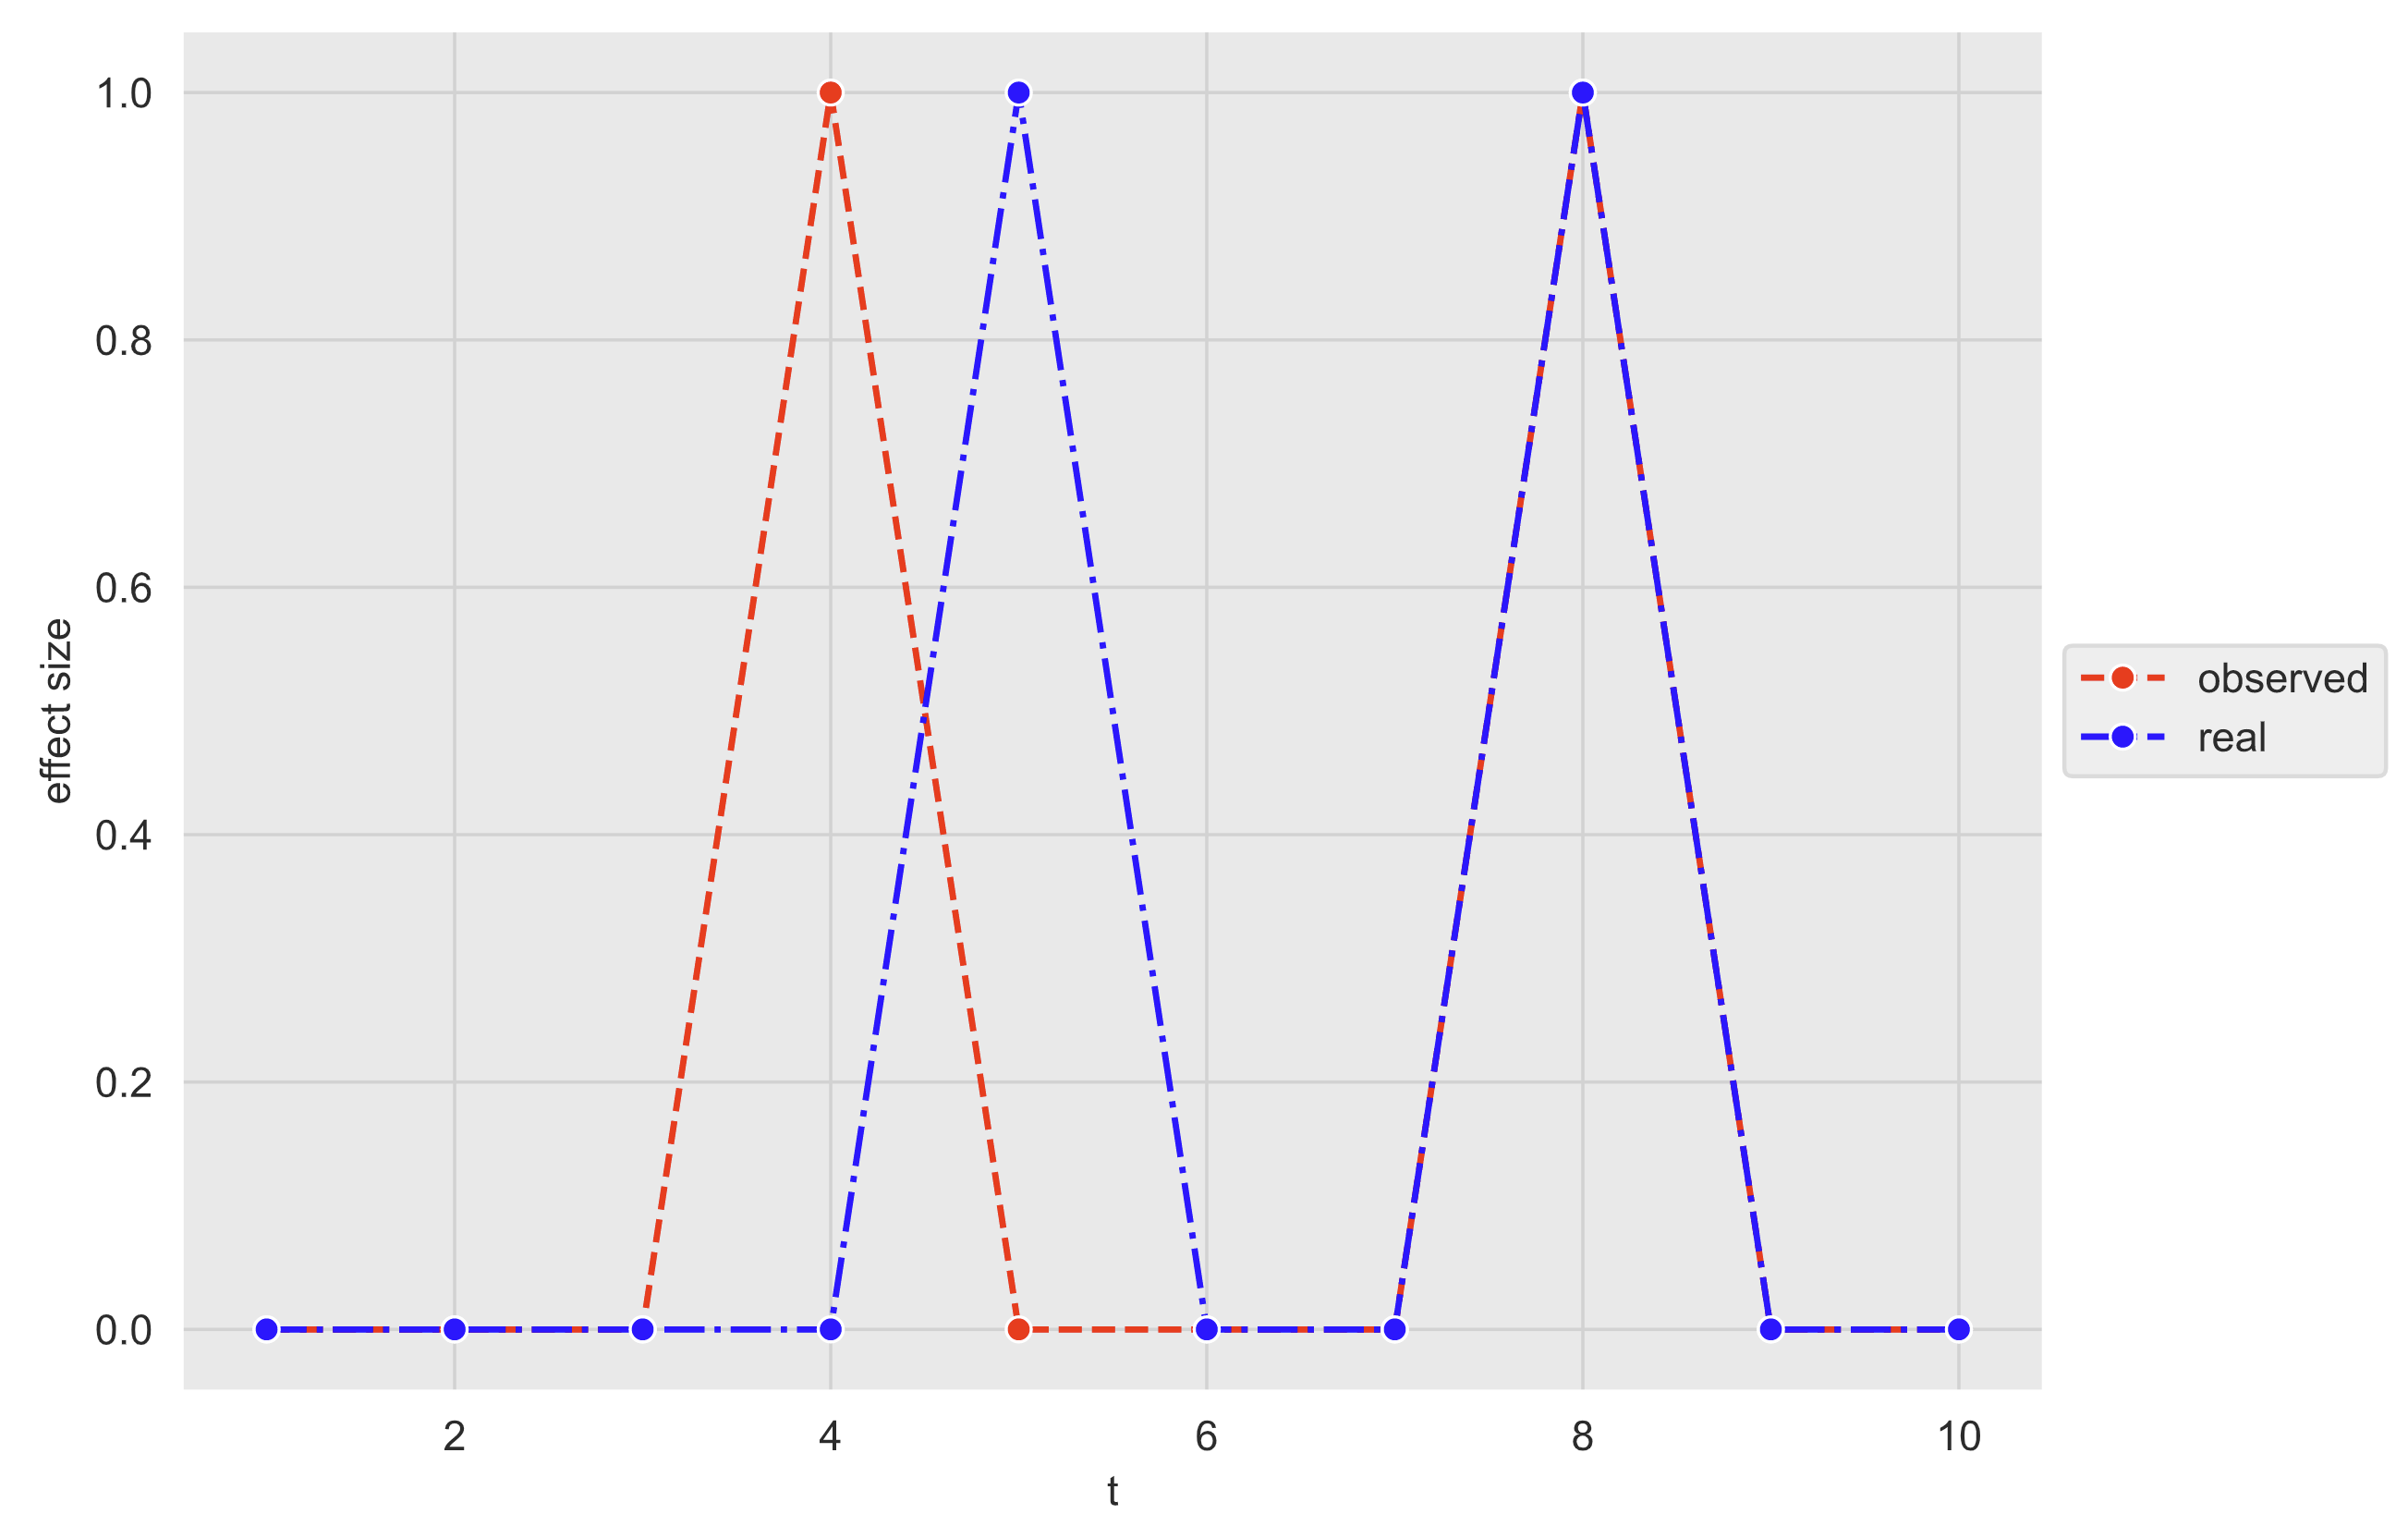
\includegraphics[totalheight=6cm]{images/2_input_delay_example.png}
\caption{Add figure caption}
\label{fig:verticalcell}
\end{figure}
\end{center}

If one were to model the effect using a fixed time delay and OLS, the estimate would only be half the true value because only one of the outputs is aligned. Obviously, this isn't ideal, we want the parameter estimates to be as close to the real values as possible, regardless of any noise in the lag structures. One can mitigate the problem via time aggregations, however in complicated multivariate cases, this is just not feasible.

Therefore, we propose a regression model which can handle stochastic time delay structures. We treat the stochastic time delay components as an ‘error’ in the time axis. Next, we find the maximum likelihood estimate, for a given set of parameters, considering the time error ($t$-axis) and the regression error ($y$-axis) simultaneously.


\section{Methodology}

We consider the problem as analogous to the typical error-in-variables (EIV) regression. Ordinary regression analyses (and machine learning models) define the loss function with respect to errors in the y axis only. For EIV, errors are considered in both the $y$-axis and the $x$-axis (REF). This is useful when there are measurement errors in the independent variable eg. because your physical measurements have some degree of random error. Similarly, for this problem we assume that we have errors in the $y$-axis and the $t$-axis. That is, there are random prediction errors and random errors in the time domain. 

Let $x: [a, b] \longrightarrow \mathbb{R}$ be a discrete time series with finite domain and we want to determine the injective, functional relationship $f$ to some other variable y. The series $x(t)$ must be a stationary series with a known value for the point at which $f(x(t)) = 0$.  That is, we know at which point the input series has no effect on the output (when it’s off). 

% TODO: Rewrite concrete expression of support...is it on x ot t? -- Aaron: f(x(t)). Consider x(t) = 0.1 for t is odd, 1 for t is even. If f(x(t)) = 0 for t is odd, 1 for t is even then the series is still valid for our method.  
\textcolor{red}{For clarity, as per convention, we use the nomenclature ‘support’ for the elements $f(x(t)) \neq 0$}. The size of the support of f(x(t)) should be small relative to the total vector length. We utilise the terminology 'impulse' for an individual element of the support set.

We also assume that the set of $\tau$'s, denoted $\mathcal{T}$, is not a constant, but rather a random draw from some discrete distribution (e.g. discrete gaussian, poisson etc). For the discrete gaussian kernel $\mathcal{T}\sim T(0, \sigma)$ or for the poisson distribution $\mathcal{T}\sim Pois(\lambda)$ and $\varepsilon \sim N(0, \sigma_{\varepsilon})$. 

Firstly, let us take the input series $x(t)$ and decompose it into its constituent non-zero impulse components. So, if $x(t)$ is a vector given by 

\begin{align}
x(t) = 
\left(
\begin{array}{cccccc}
0 & 0 & 1 & 0 & 1 & 0
\end{array}  
\right)
\end{align}

then we decompose the vector into a matrix 

\begin{align}
X(t) = 
\left(
\begin{array}{cccccc}
0 & 0 & 1 & 0 & 0 & 0 \\
0 & 0 & 0 & 0 & 1 & 0 
\end{array}  
\right)
\end{align}

where each impulse is treated separately. \\

Our algorithm then attempts to find the maximum likelihood estimate for the following equation:

% TODO fix notation for T
\begin{align}
y(t)= f(X(t + \mathcal{T})) + \varepsilon
\end{align}

where $X(t + \mathcal{T})$ is the matrix of time shifted impulses and $X(t)$ is the observed input.\\

In order to find the best estimate of $f$, we would like to find the function $f$ which maximises the joint likelihood of both Tau(?) and $\varepsilon$, the time-domain likelihood and the error likelihood respectively.

Specifically, we maximise the log-likelihood of the following relation:
% TODO: Clean this notation.
\begin{align}
\max  \left( \log \left(\mathcal{L}(\theta_{\varepsilon}, \varepsilon) \times \mathcal{L}(\theta_{\tau}, \tau)\right) \right)
\end{align}

where $\theta_{\varepsilon}$ and $\theta_{\tau}$ represent the parameters of the prediction error and time error respectively. For simplicity, assume that the tau and error distributions are independent. To begin with, the values of each individual time shift ($\tau$) are not known. In addition, prediction error distribution $\varepsilon$ can only be determined if each $\tau$ is known (because for each time shift there is a different prediction and prediction error). Therefore, our algorithm finds the optimum set of time shifts  in an inner optimisation, while iteratively searching for the optimum parameters of $f$ in an outer optimisation step. 

\section{Algorithm}

Firstly, we define a parametric form and some initial parameters to be estimated for the function $f$. For simplicity, let's take the univariate linear model where the $f(x(t))$ is parameterised by $\beta$, $\sigma_{\varepsilon}$(error standard deviation)  and $\sigma_{\tau}$ (time error standard deviation). First, we initialise some starting values for each of these parameters.

Now, we want to find the best possible time shift $\tau$ for each input impulse in $X(t)$. It stands to reason that the best possible time shift would be one that is not too far away from the observed impulse and also gives the best possible prediction. In this example, we can calculate the prediction 'y' by simply multiplying the shifted value by its parameter $\beta$. From there, the likelihood estimate is derived from the time shift and the prediction error.

In principle, we can iterate over a number of values of $\tau$ (i.e. optimise) until we maximise the likelihood for the specific impulse.

However, we must also consider that the impulses in $X(t)$ are not independent from each other. After shifting, it's possible that two or more effects occur simultaneously.

This is particularly problematic if there are multiple impulses within a short period of time, or impulses have a distributed effect over multiple time points. 

As an example consider the series 

\begin{align}
x(t) = 
\left(
\begin{array}{cccccc}
0 & 0 & 1 & 1 & 0 & 0
\end{array}  
\right)
\end{align}

with $\mathcal{T}= (1, 0)$ and $\beta = 1$. For this case, 

\begin{align}
X(t + \mathcal{T}) = 
\left(
\begin{array}{cccccc}
0 & 0 & 1 & 0 & 0 & 0 \\
0 & 0 & 1 & 0 & 0 & 0 
\end{array}  
\right)
\end{align}

and the effect is therefore 
\begin{align}
y = 
\left(
\begin{array}{cccccc}
0 & 0 & 0 & 2 & 0 & 0
\end{array}  
\right)
\end{align}

To accurately calculate the likelihood, we must optimise the time shifts simultaneously.

Therefore, we treat the problem of finding the best set of time shifts as a discrete optimisation problem.

For the optimisation step we utilise two assumptions. Firstly, smaller shifts are more likely than larger shifts (proportionate to the standard deviation of the $\mathcal{T}$ distribution). The algorithm should explore the space of smaller shifts more often than larger shifts. Secondly, impulses close to each other are more likely to be dependent than impulses further away. 

We initialize the optimisation algorithm with all parameters set to the mean of the $\mathcal{T}$ distribution (e.g. zero for the zero mean gaussian). Next, we randomly select a small number of impulses, with the value treated as a hyperparameter. The shifts are then randomly changed to a value drawn for the T distribution (proposal vector), and the likelihood (both time shift and prediction error) for the proposal is calculated. If the proposal likelihood is higher than the current maximum likelihood, we update our initial estimate to the current best guess. This procedure is done in a loop with the best guess of the set of T improving over time.

Lastly, we optimise over the set of parameters $\beta$, $\sigma_{\varepsilon}$ and $\sigma_{\tau}$, iteratively alternating between the time shift optimisation and the parameter optimisation. For the parameter optimisation, typical methods such as gradient descent, genetic algorithms or annealing can be used.  In our implementation we have used the differential evolution algorithm from scipiy.optimize (REF), because of its ability to handle noisy objective functions. In order to improve convergence, we also standardize all input variables to the range 0-1.

Through optimisation, we find the best fit for the values of $\beta$, $\sigma_{\varepsilon}$ and $\sigma_{\tau}$. The accuracy of the final parameter estimate is relative to the ratio of the $y$-axis error and the effect size $\beta X(t)$. As $\sigma_{\varepsilon}/(\beta X(t))$ tends to infinity, the estimated value of $\sigma_{\tau}$ tends to zero. In the event that $\sigma_{\tau}=0$, the model becomes a ‘fixed lag’ model, and for the discrete gaussian case the parameter estimate $\beta$ tends to the standard linear regression coefficient.
On the other hand as $\sigma_{\varepsilon}/(\beta X(t))$ tends to zero, the coefficient estimate tends to the true value. Therefore, the method provides no guarantee on recovering the exact time shifts, only that the estimates are equal to or better than their OLS counterparts.

\section{Limitations}
%TO-DO : Improve the formulas
As the length of $x(t)$ increases, more impulses are introduced and the size of the decomposed matrix $X(t)$ also increases. At some point, handling $X(t)$ becomes impractical. To account for this, we assume that distant impulses do not affect each other. Concretely, for the $ith$ and $j_th$ impulse (row) in $X(t)$, separated by time $t$, the effect vectors $f(X_i(t + \tau_i))$ and $f(X_j(t + \tau_j))$ are linearly independent.

Therefore, the matrix $X(t)$ is decomposed into a number of segments, where each segment is 
composed of a smaller number of dependent impulses. To select the right split locations, we search the time series for locations with the lowest impulse density. Given that we wish to split $X(t)$ into independent matrices $U_n(t)$ and $V_m(t)$, 
if we choose the split locations such that $\forall_i$ $\epsilon$ $n$ and  $\forall_j$ $\epsilon$ $m$, 
$f(U_i(t + \tau_i))$ is linearly independent from $f(V_j(t + \tau_j))$, 
then segments will also be independent and the procedure unique. 
In practice, it may not be possible to guarantee complete independence of every segment, 
in which case results may vary. After segmentation, each matrix can be optimised independently, 
in parallel, making the inner optimisation procedure tractable for longer length sequences. 

Finally, a note on problem constraints. The likelihood estimates are dependent on the inner ($\mathcal{T}$) optimisation procedure. There is no guarantee that the global maximum will be found during this process, particularly for sequences with a high density of impulses. 

For example, consider the example sequence 

\begin{align}
    x(t) = 
    \left(
\begin{array}{cccccccccc}
    0.5 & 0.6 & 0.4 & 1 & 2 & 1 &
    0.3 & 0.2 & 0.5 & 0.8 
\end{array}  
\right)
\end{align}

where each impulse can shift between -2 and +2 positions. Ignoring shifts beyond the edge of the vector, the solutions space of $\mathcal{T}$ is $5^t$ combinations.  
In such cases, the estimated likelihood is likely to be close to but not exactly the same as the real value. As the density (in time) of impulses increases, the accuracy of the estimates decrease. Therefore, this model is most appropriate for sparse time series inputs.

\section{Experiment}

The following section demonstrates a simulated univariate example. Full code to reproduce the example can be found via \href{https://github.com/aaron1rcl/tvs_regression/}{TVS Regression on GitHub}.

Figure \ref{fig:simulated_example} shows the simulated time series.

The input signal has 17 non-zero impulses which have been drawn from the standard normal distribution. The system is 'off' when $x(t) =0$. In other words, when $x(t) = 0$, $f(x(t)) = 0$. 

The true shift distribution $\mathcal{T}$ is given by $\mathcal{T}$ $~ N(0, 2)$. There is one value of $\tau$ for each of the 17 impulses.

The green line represents the shifted series, corresponding to the time at which the effect occurs. The blue line is the output ‘y’.

The values for the parameters were arbitrarily selected. The output y is defined by the following equation:


\begin{align}
    y = 2X(t + \mathcal{T}) + 6.5
\end{align}


\begin{center}
\begin{figure}
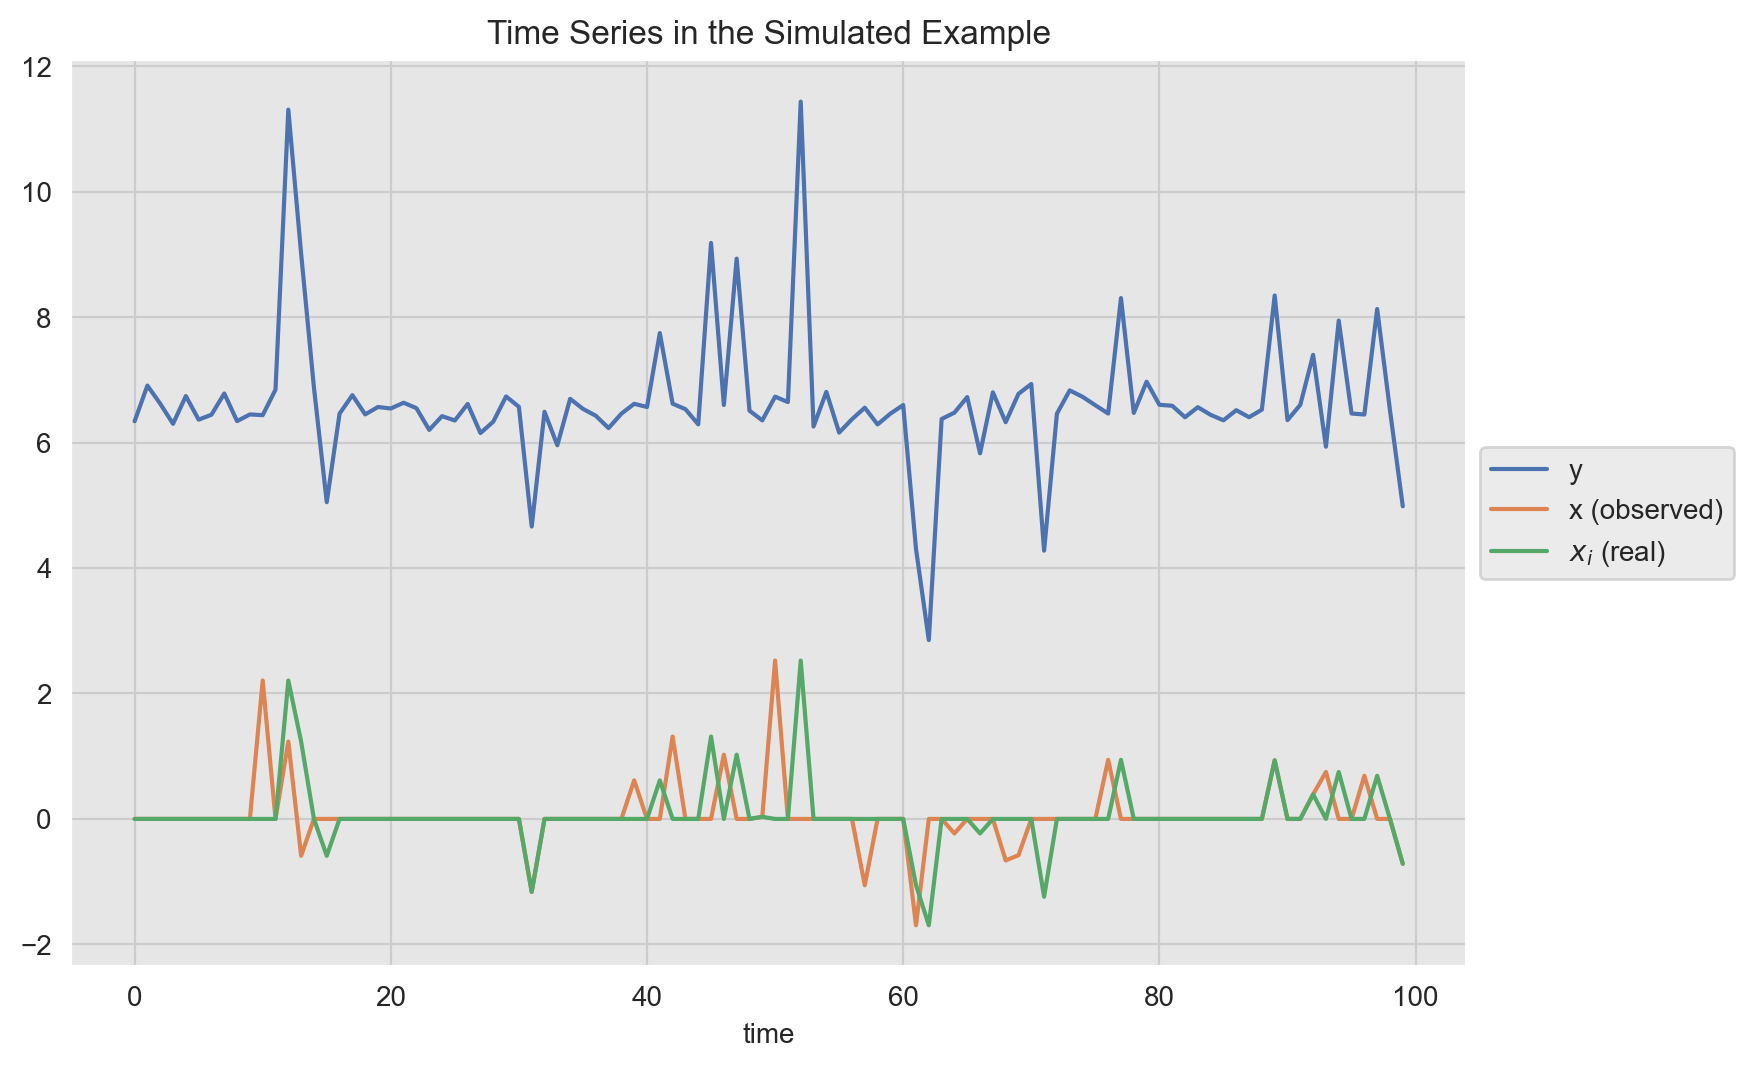
\includegraphics[scale=0.5]{images/simulated_example.png}
\caption{Simulated Example Data}
\label{fig:simulated_example}
\end{figure}
\end{center}

A histogram of the actual distribution of $\mathcal{T}$ is shown in Figure \ref{fig:real_shifts}.

\begin{center}
\begin{figure}
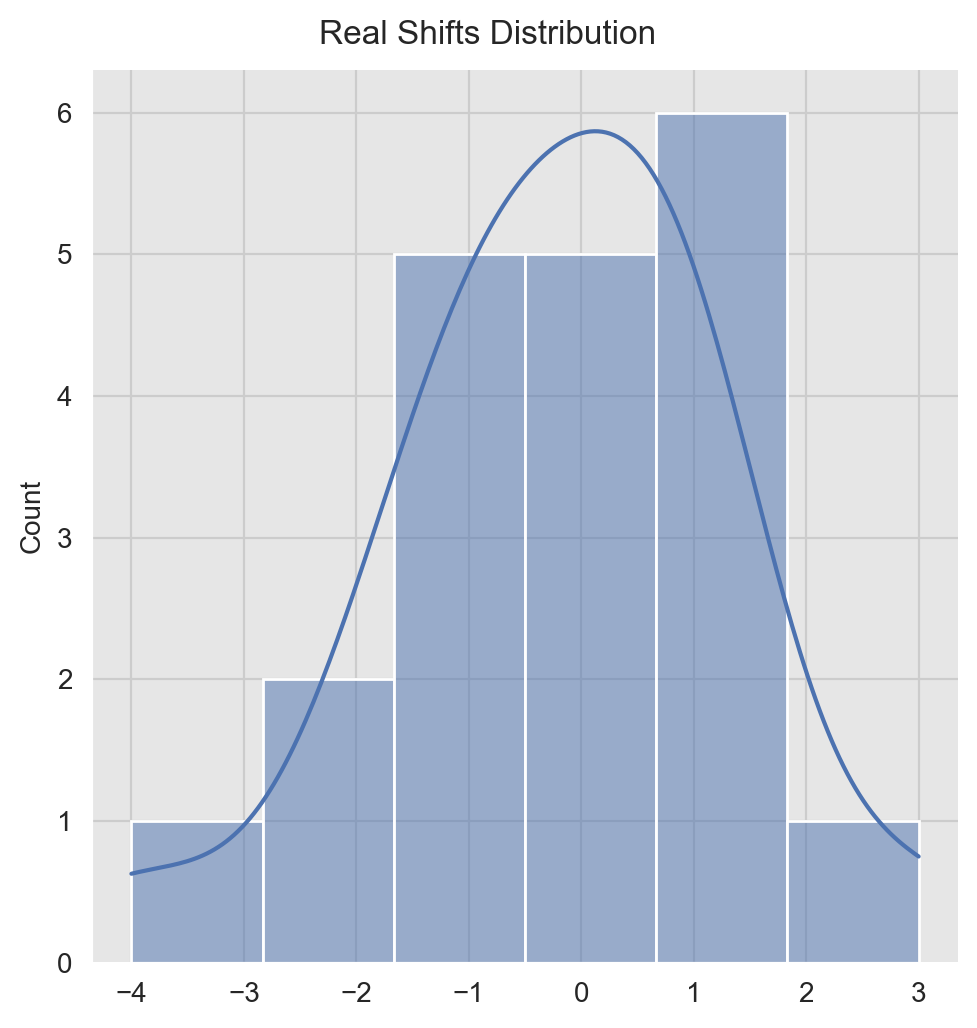
\includegraphics[scale=0.5]{images/real_shifts.png}
\caption{Real Shift Distribution $\mathcal{T}$.}
\label{fig:real_shifts}
\end{figure}
\end{center}

After fitting the model, we obtain the following results. Figure \ref{fig:tvs_ols_fit} show the model fit (denoted TVS) and a comparison with standard OLS. Figure \ref{fig:tvs_errors} and Figure \ref{fig:convergence} show the errors distribution of the TVS fit and  convergence of the TVS model respectively.

\begin{center}
\begin{figure}
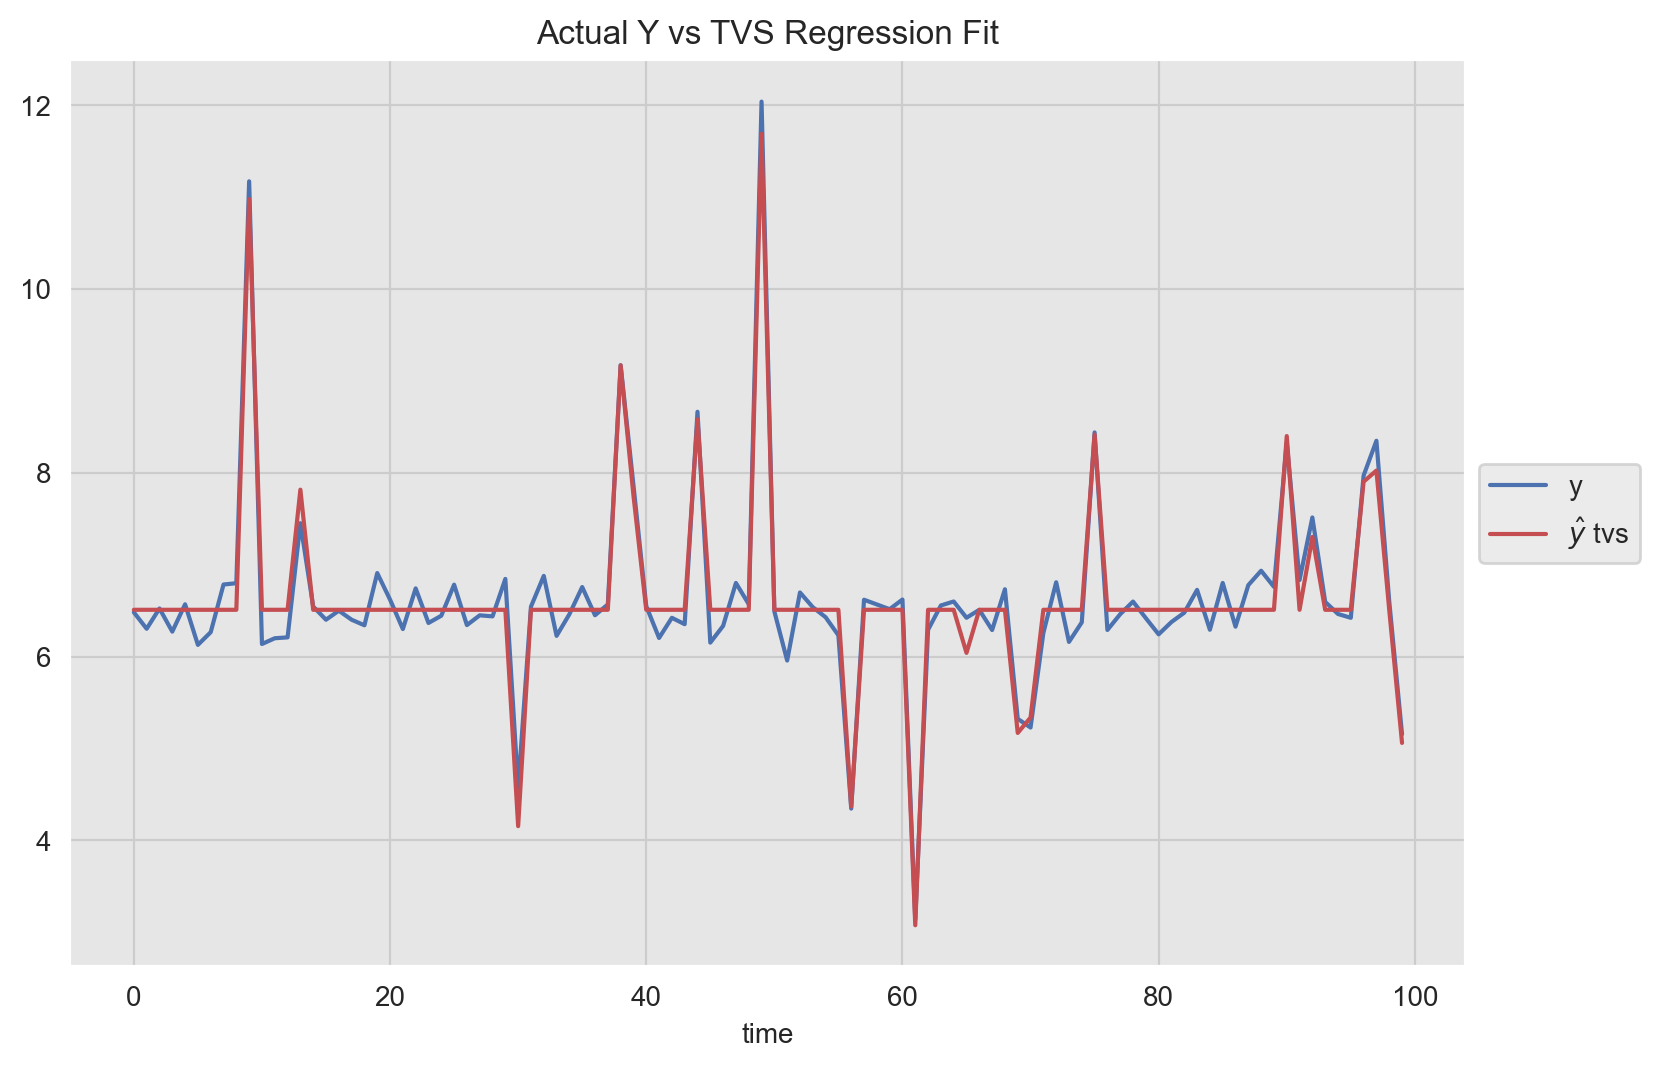
\includegraphics[scale=0.6]{images/tvs_fit.png} 
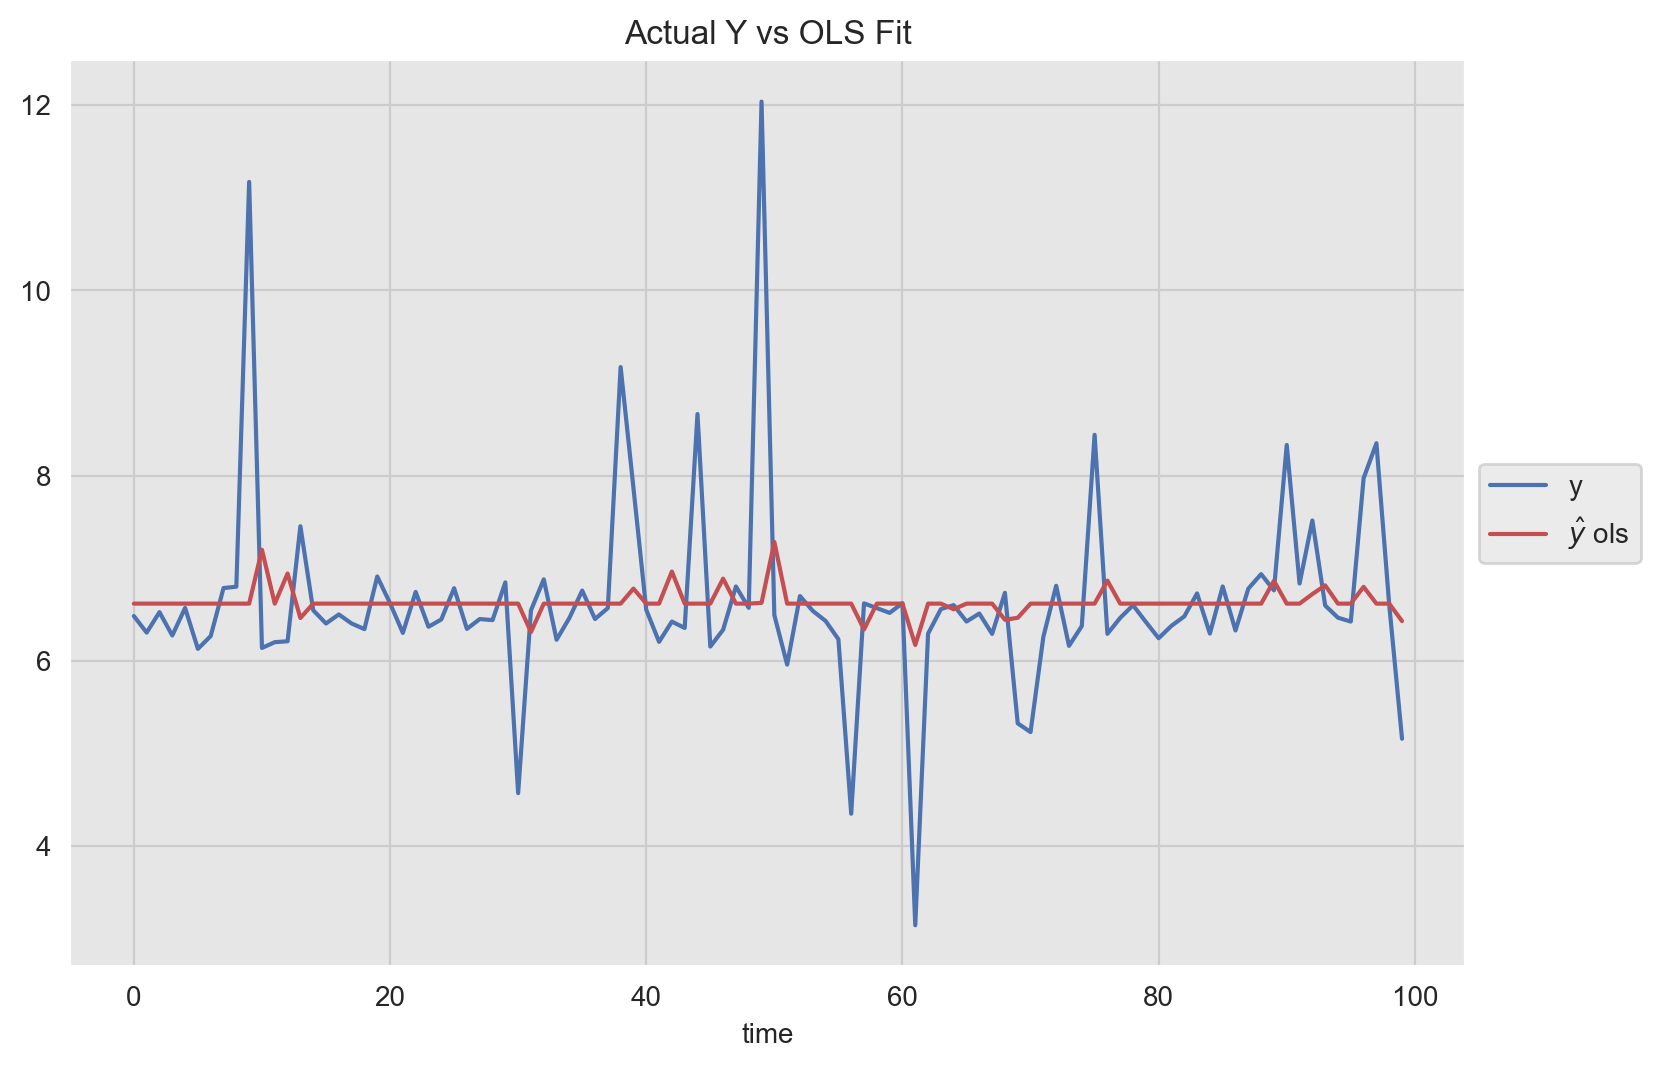
\includegraphics[scale=0.3]{images/ols_fit.png} 
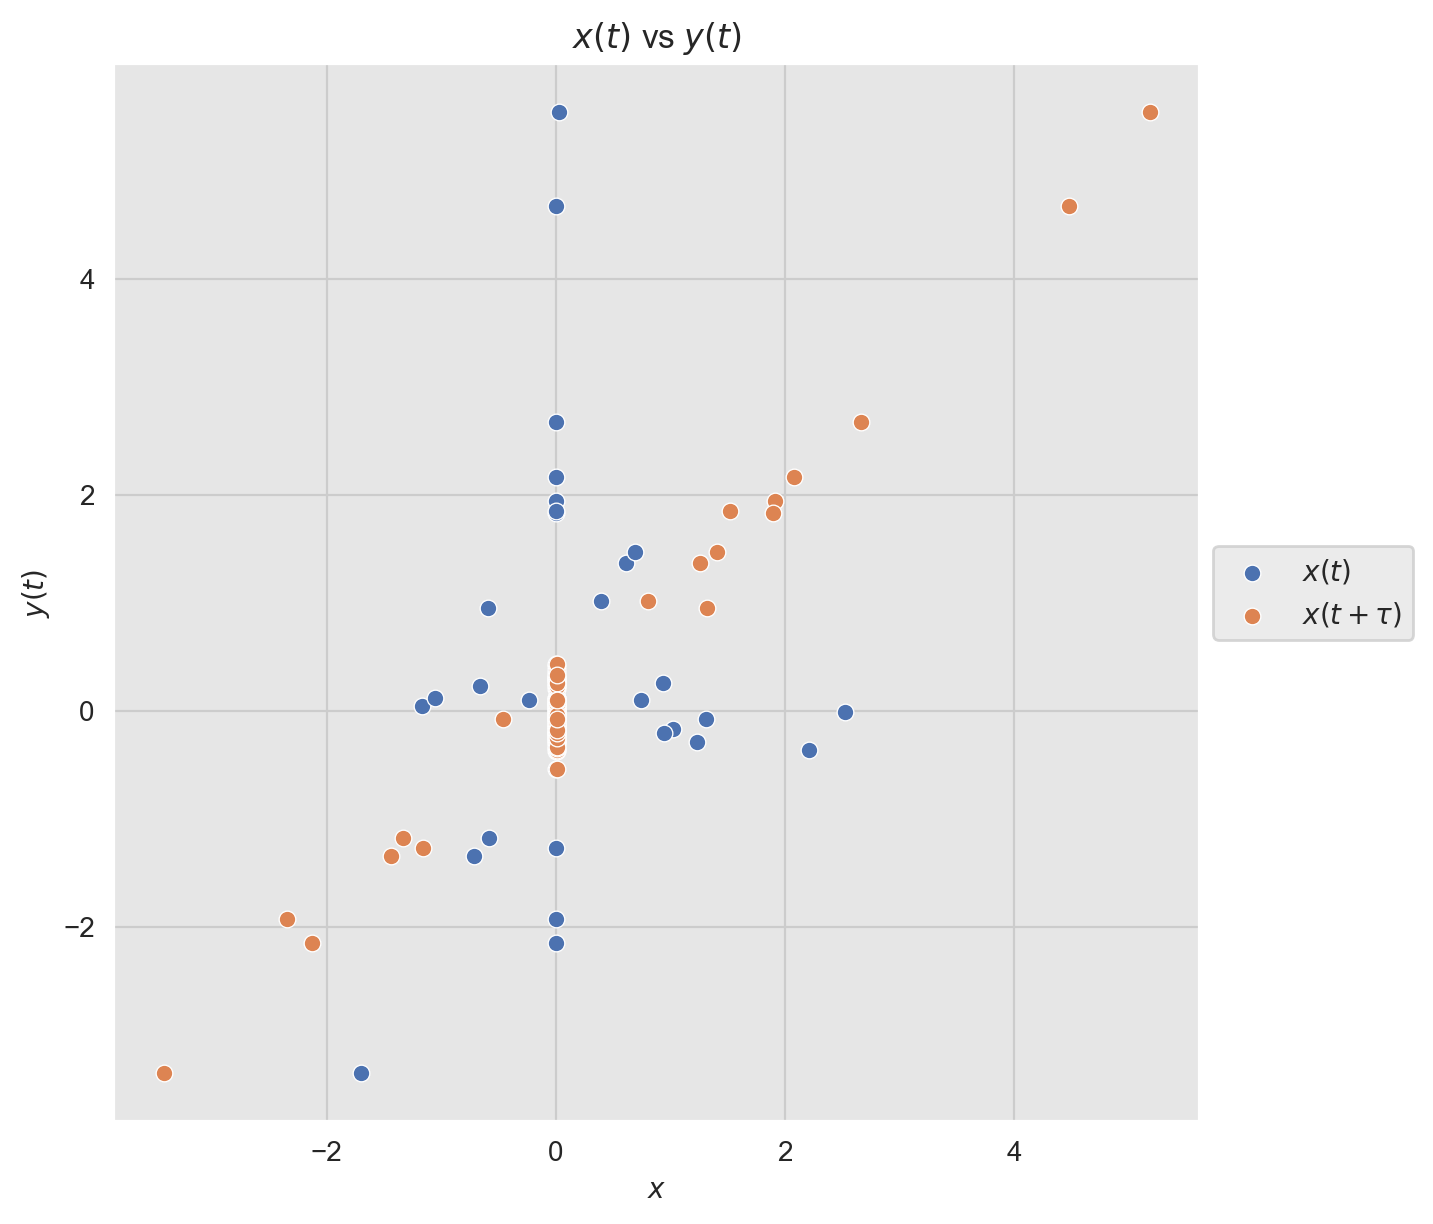
\includegraphics[scale=0.3]{images/scatterplot.png} 
\caption{TVS vs OLS model fit.}
\label{fig:tvs_ols_fit}
\end{figure}
\end{center}

\begin{center}
\begin{figure}
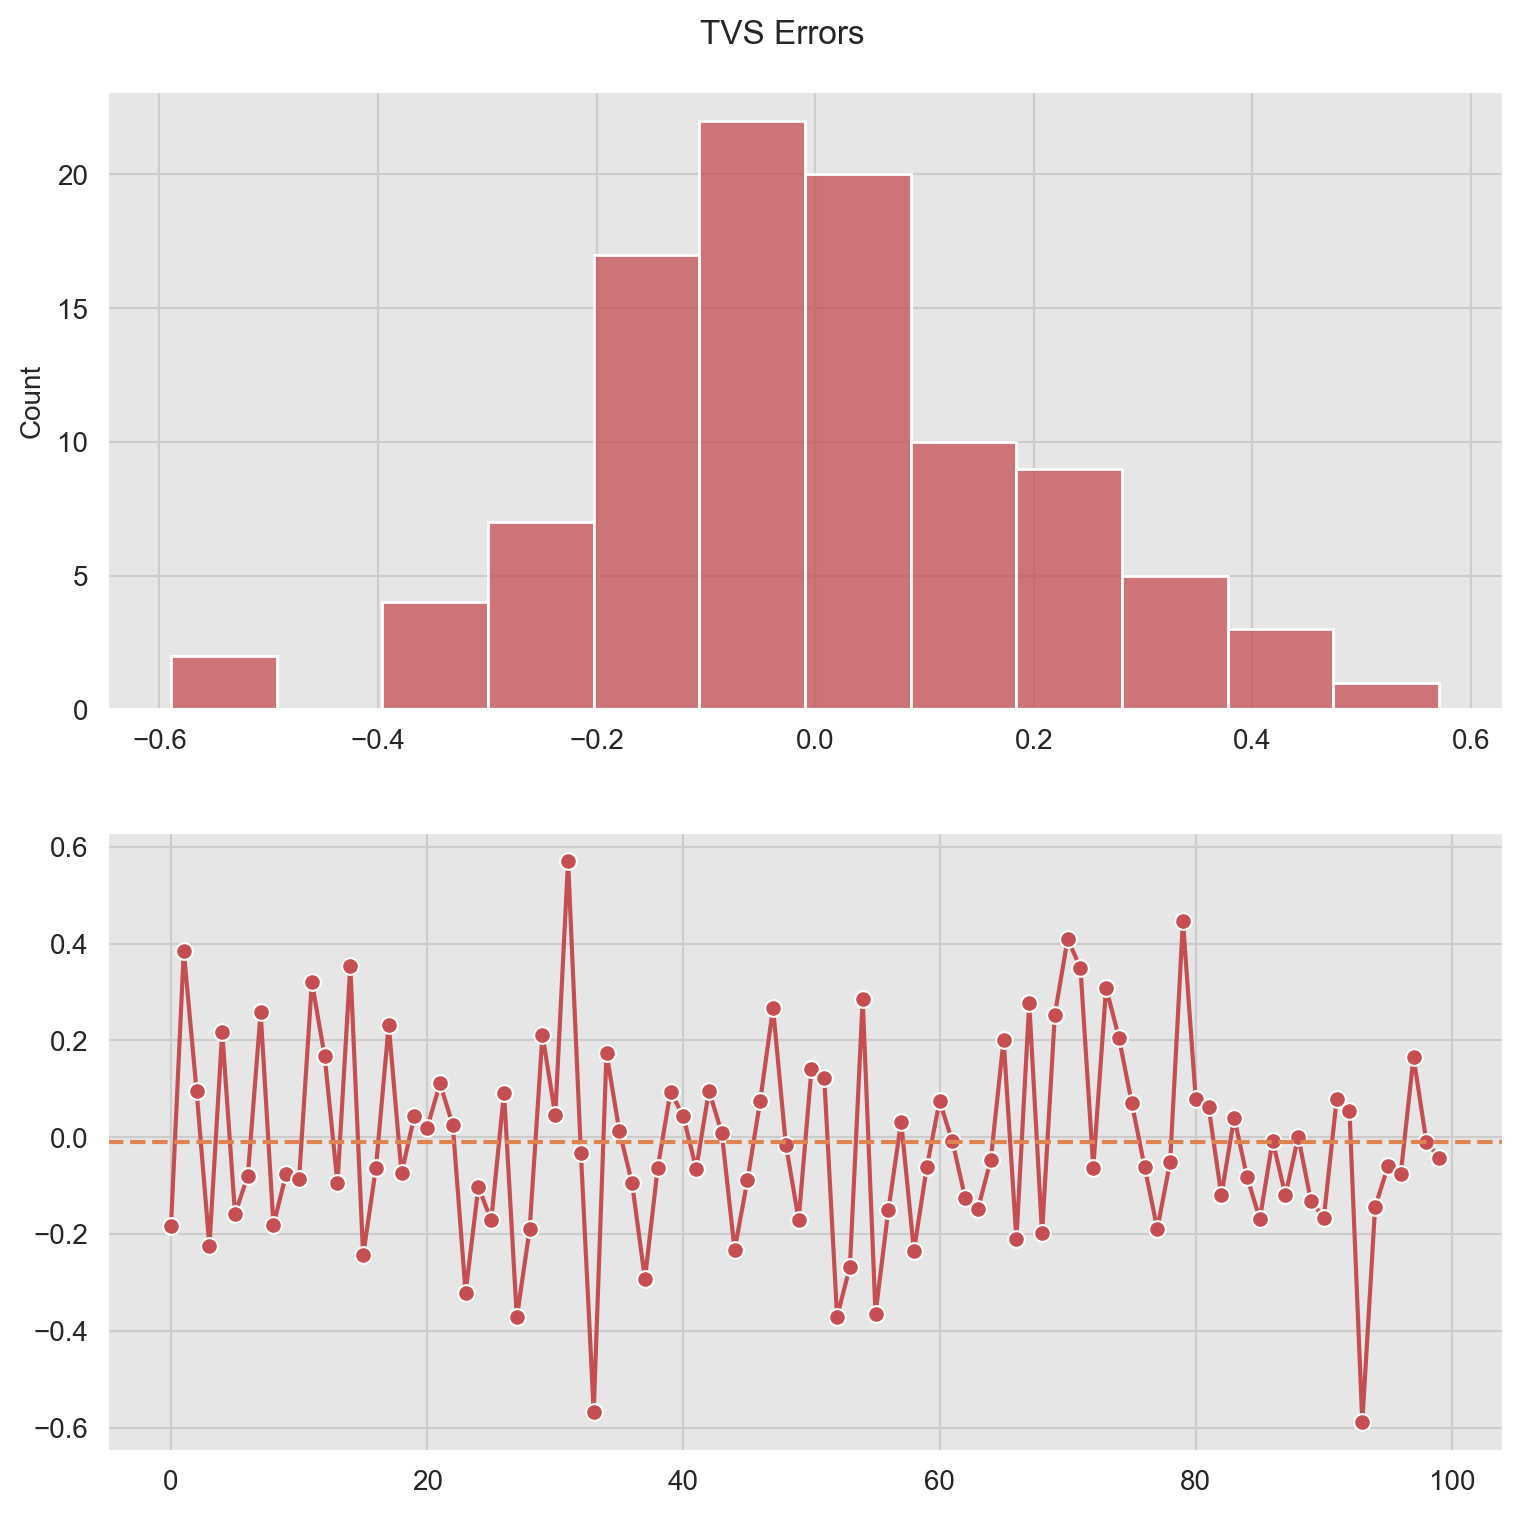
\includegraphics[scale=0.5]{images/tvs_errors.png}
\caption{Errors...}
\label{fig:tvs_errors}
\end{figure}
\end{center}

\begin{center}
\begin{figure}
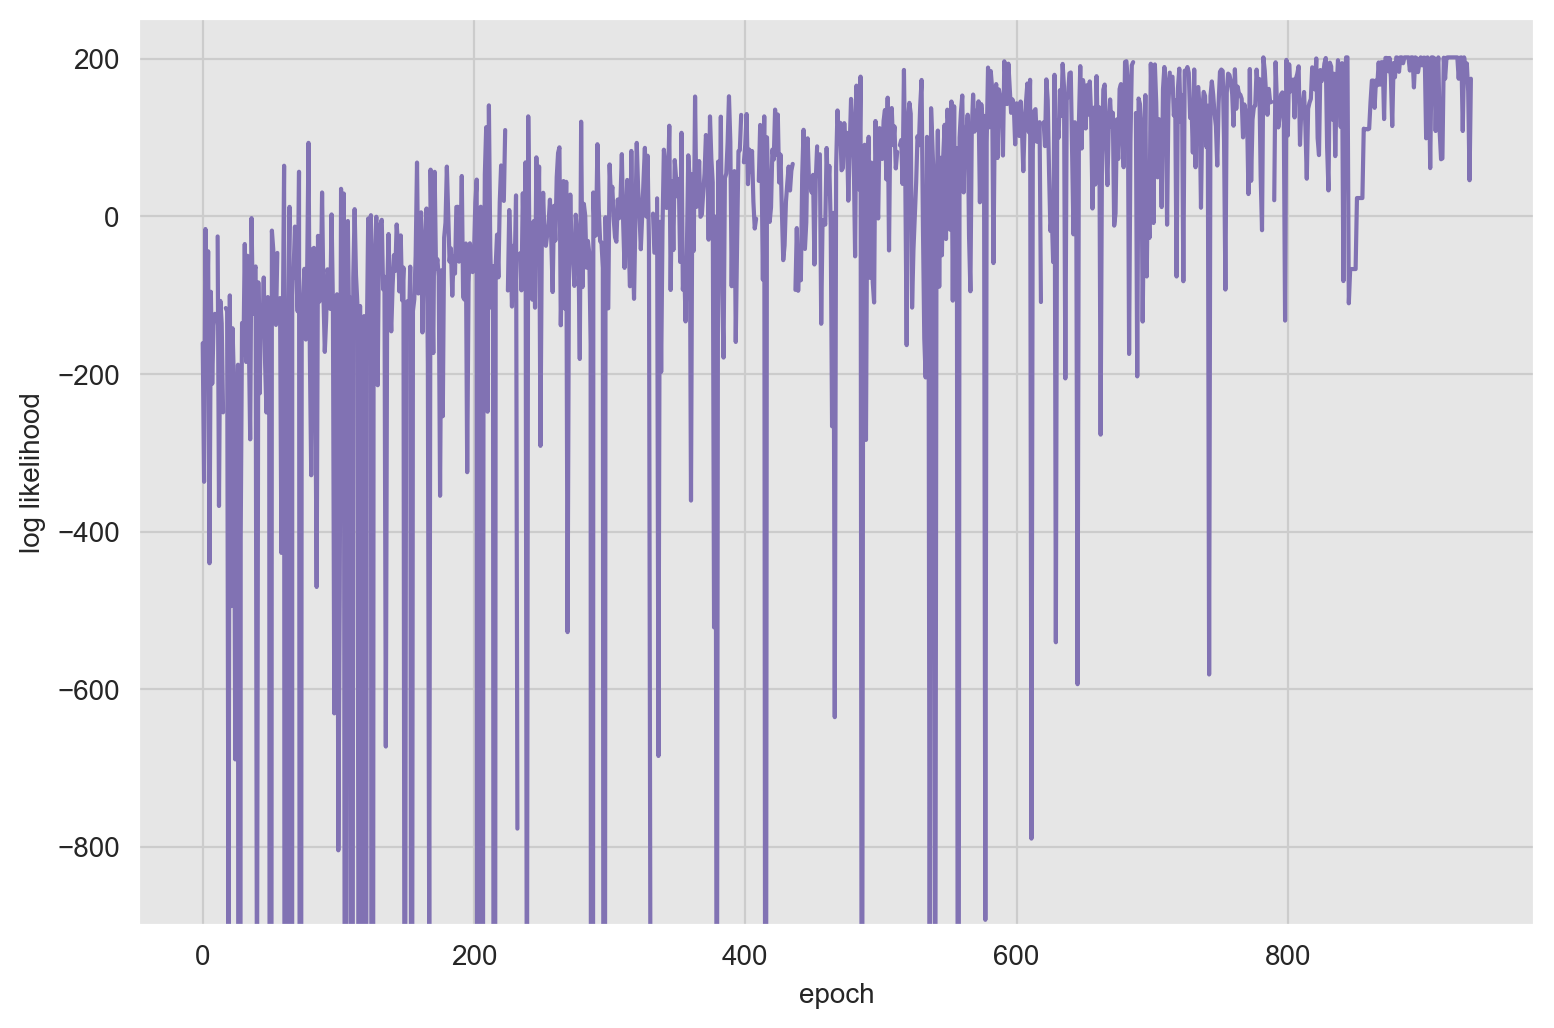
\includegraphics[scale=0.6]{images/convergence.png} 
\caption{Convergence ...}
\label{fig:convergence}
\end{figure}
\end{center}

The true set of $\mathcal{T}$ is:

\begin{align}
\mathcal{T} = 
\left(
\begin{array}{ccc}
-1 & 1 & 0 
\end{array}  
\right)
\end{align}

Compared to the estimated $\mathcal{T}$:

\begin{align}
\mathcal{T}_{est} = 
\left(
\begin{array}{ccc}
-1 & 1 & 0 
\end{array}  
\right)
\end{align}

%To-do - write in the actual T distributions above. Not sure how to fix the hbox problem.


%To-do properly format the table
\begin{tabular}{c|c|c|c|}
\hline
Parameter & TVS Regression & OLS Regression & True Value \\
\hline
$\beta$ & 1.96 & 0.26 & 2  \\
\hline
$Intercept$ & 6.48 & 6.62 & 6.5 \\
\hline
$\sigma_t$ & 1.51 & $N/A$ & 1.47 \\
\hline
$\sigma_e$ & 0.26 & 1.03 & 0.2 \\
\end{tabular}

As shown above, the estimated values for $\beta$ and $\sigma_e$ are significantly improved by taking into account the stochastic time delay noise. The estimated $\beta$ using OLS regression is 0.25, compared to the true value 2. Even a small amount of noise in the time axis causes attenuation, 
limiting the usefulness of OLS for these problems.
In comparison, the algorithm described herein estimates a $\beta$ of 1.96, much closer to the true value.

While the example is based on simulated data, we believe that the experiment demonstrates clear potential for improvement in the modelling of real world systems with stochastic time delay noise.


\section{Future Work}

In the univariate case, the utility of the described method is limited. However, we propose three extensions as future work. The first is to extend the method to multiple regression. We believe that the extension can be built on the same fundamental ideas presented in this document. Next, the model could be extended to include distributed lag structures. A distributed lag structure is where past values of the impulse influence future values of the output. Finally, in relating $x(t)$ to $f(x(t))$, the function f could be extended to the modelling of non-linear forms.

Through these extensions we can begin to tackle a larger number of practical problems.

In addition, by incorporating these elements we could begin to explore alternative forms of time series prediction. Essentially, existing prediction mechanisms predict the average across time shifts.However, in some situations the predictions could be considered nonsensical.

For example, let us consider a regression model to predict how much coffee someone drinks between 9am and 9:30am, at work. They set off every day in their car at exactly 8:30am and it takes about 30 minutes (+- $\tau$) to get to work. The time shift $\tau$ could be caused by something as simple as variations in traffic. When they get to work, they always have a coffee. A typical regression might predict $0.5$ coffees between 8:30 am and 9am and $0.5$ coffees between 9am and 9:30am. Alternative prediction forms such as: 'When they get to work, they will have 1 coffee' might be more useful.


\section{Conclusion}

We have proposed a form of regression analysis suited to the modelling of stochastic time delay problems. In addition, we have shown the feasibility of the approach and its performance on simulated data. Our approach allows for consistently improved estimation and prediction when the input is affected by noise in the time domain. To our knowledge, the method is novel for this class of problem.


\end{document}